% Docummentation: 
% - https://www.latex-project.org/help/documentation/
% - https://docs.w3cub.com/latex/
% - https://tex.stackexchange.com/questions/455993/formatting-sql-code
%   https://www.overleaf.com/learn/latex/Code_listing#Code_styles_and_colours

\documentclass[a4paper,10pt]{report}

\usepackage{polski}         % Polish diacretic signs
\usepackage[utf8]{inputenc} % required for international characters
\usepackage{hyperref}       % urls and hyperlinks
\usepackage{xurl}           % break urls
\usepackage{microtype}      % improve justification
\usepackage{enumitem}       % compact lists
\usepackage{graphicx}       % Include graphics
\usepackage{wrapfig}        % wrap text aroung graphics
\usepackage{fancyhdr}       % Customize page layout
\usepackage{index}          % Create an index
\usepackage{setspace}       % Spacing
\usepackage{float}          % Forcing figure placement
\usepackage{tabularray}     % Tables with wrapping
\usepackage{xcolor,listings}% Code listings
\usepackage{textcomp}       % Code listings
\usepackage{color}          % Code listings
\makeindex
\graphicspath{ {./} }       %Was ./figures/ changed so i can peek in VS Code


% Code listings
\definecolor{codegreen}{rgb}{0,0.6,0}
\definecolor{codegray}{rgb}{0.5,0.5,0.5}
\definecolor{codepurple}{HTML}{C42043}
\definecolor{backcolour}{HTML}{F2F2F2}
\definecolor{bookColor}{cmyk}{0,0,0,0.90}  
\color{bookColor}

\lstset{upquote=true}

\lstdefinestyle{mystyle}{
    backgroundcolor=\color{backcolour},   
    commentstyle=\color{codegreen},
    keywordstyle=\color{codepurple},
    numberstyle=\numberstyle,
    stringstyle=\color{codepurple},
    basicstyle=\footnotesize\ttfamily,
    breakatwhitespace=false,
    breaklines=true,
    captionpos=b,
    keepspaces=true,
    numbers=left,
    numbersep=10pt,
    showspaces=false,
    showstringspaces=false,
    showtabs=false,
}
\lstset{style=mystyle}

% Code listings
\newcommand\numberstyle[1]{%
    \footnotesize
    \color{codegray}%
    \ttfamily
    \ifnum#1<10 0\fi#1 |%
}

% ------------------------------ Custom Commands ------------------------------
% Usage: \command\{text}  
\newcommand{\customstyletitle}[1]{\Huge{\textbf{#1}}}
\newcommand{\customstylechapter}[1]{\large{\textit{#1}}}
\newcommand{\customstylesection}[1]{\textbf{\textit{#1}}}
\newcommand{\customstylesidenote}[1]{\Small{\textbf{#1}}}
\newcommand{\customstyletable}[1]{\footnotesize{\textbf{#1}}}
\newcommand{\customstyletablecentered}[1]{\footnotesize\centering{\textbf{#1}}}
\newcommand{\customstyleindivisible}[1]{
    \begin{minipage}{\textwidth}
        {#1}
    \end{minipage}
}

\lstnewenvironment{SQLlisting}[2][]%
  {\noindent\minipage{\linewidth}\medskip
   {#2}
   \smallskip
   \lstset{basicstyle=\ttfamily\footnotesize,
            frame=single,
            language=SQL,
            deletekeywords={IDENTITY},
            %deletekeywords={[2]INT},
            morekeywords={clustered},
            framesep=8pt,
            xleftmargin=40pt,
            framexleftmargin=40pt,
            frame=tb,
            framerule=0pt,
            caption=#1}}
  {\endminipage}

  % spacer
\newcommand{\HRule}{\rule{\linewidth}{0.5mm}} % horizontal lines



% --------------------------- documment starts here ---------------------------

% environment
\begin{document}

% Define pagestyle
% [REQUIREMENT] 23. Przypisy dolne, stopki (nr stron), nagłówki...
\pagestyle{fancy}
\fancyhf{}          %clears default headers and footers
\renewcommand{\headrulewidth}{2pt}
\renewcommand{\footrulewidth}{1pt}

\fancypagestyle{mychapterpage}{%
    %\fancyhead[LE]{\leftmark}
    %\fancyhead[RO]{\rightmark}
    \fancyfoot[RO,LE]{\thepage}
    \renewcommand{\headrulewidth}{2pt}
    \renewcommand{\footrulewidth}{1pt}
}


% https://texblog.org/2013/09/16/multiple-page-styles-with-fancyhdr/
%Redefine chapter by adding fancy as the chapter title page page-style
\makeatletter
    \let\stdchapter\chapter
    \renewcommand*\chapter{%
    \@ifstar{\starchapter}{\@dblarg\nostarchapter}}
    \newcommand*\starchapter[1]{%
        \stdchapter*{#1}
        \thispagestyle{mychapterpage}
        \fancyfoot[RO,LE]{\thepage}
        \markboth{\MakeUppercase{#1}}{}
    }
    \def\nostarchapter[#1]#2{%
        \stdchapter[{#1}]{#2}
        \thispagestyle{mychapterpage}
        \fancyfoot[RO,LE]{\thepage}
    }
\makeatother


% [REQUIREMENT] 1. Strona tytułowa
\begin{titlepage}
	%---Headings------------------------------------------	
	\begin{center}
    \begin{onehalfspace}
    \textsc{\LARGE{WYŻSZA SZKOŁA TECHNOLOGII INFORMATYCZNYCH W KATOWICACH}}\\
    \end{onehalfspace}
    \textsc{\large{WYDZIAŁ INFORMATYKI}}\\
	\textsc{\large{KIERUNEK: INFORMATYKA}}\\
    \end{center}
    
    %---Author--------------------------------------------
	\begin{flushleft}
    \textsc{Nowak Marcin}\\[0cm]
    \textsc{Nr Albumu 08255}\\[0cm]
    \textsc{Studia niestacjonarne}\\[0cm]
    \end{flushleft}
	
    %---Title---------------------------------------------
	\begin{center}
    \HRule\\[0.4cm]
	{\customstyletitle{Projekt i wdrożenie aplikacji wspomagającej zarządzanie budżetem domowym}}\\[0.4cm] 
    \HRule\\[1.5cm]
    \end{center}
	
    %---Description----------------------------------------
	\begin{flushright}
        \textsc{Przedmiot: Projekt Systemu Informatycznego}\\[0cm]
        \textsc{pod kierunkiem}\\[0cm]
        \textsc{mgr. Jacek Żywczok}\\[0cm]
        \textsc{W roku akademickim 2022/23}\\[0cm]
    \end{flushright}
 
	%---Date & logo---------------------------------------
	\vfill                  % Position the date lower
	\begin{center}
    {Katowice 2022}\\	    % \today
	
\includegraphics[width=0.2\textwidth]{figures/WSTI-logo.jpg}\\[1cm]
	\end{center}
\end{titlepage}

% [REQUIREMENT] 2. Spis treści
\renewcommand*\contentsname{Spis treści}
\tableofcontents                    % prints automatical table of contents

% ---------------------------------- Content ----------------------------------

% [REQUIREMENT] 3. Wprowadzenie do tematyki projektu
\chapter{\customstylechapter{Wprowadzenie do tematyki projektu}}
{Finanse są dziedziną nauki ekonomicznej któa zajmuje się rozporzadzaniem 
pieniędzmi \cite{wiki_ekonomia}. Nauka ta w podobnym zakresie a różnej skali 
wykorzystywana jest tak przez państwa, przedsiębiorstwa jak i zwykłych obywateli
 - w efekcie jest to dziedzina o stosunkowo prostych podstawach jednak niesamowicie
skomplikowana w każdym zakresie w którym chętna osoba zadecyduje się ją zagłębić. 
Wiedza z zakresu finansów staje się szczególnie przydatna podczas gdy na rynku 
panuje trudna sytuacja ekonomiczna, w takich warunkach nierzadko decyduje ona o 
jakości oraz stanie życia poszczególnych osób fizycznych, przedsiębiorstw czy 
państw. W przypadku państw i firma przeważnie budżetem zarządzają dedykowane 
osoby lub też całe zespoły, posiadające ekspercką wiedze w dziedzinie finansów. 
Jednak osoby zarządzające budżetem domowym najczęściej dysponują wyłacznie 
nabytym doświadczeniem, rzadko jeśi wogóle wspomagając się jakimikolwiek 
narzędziami które ułatwiałyby to zadanie.}
%
% [REQUIREMENT] 4. Zamierzony cel projektu
\chapter{\customstylechapter{Zamierzony cel projektu}}
{Celem projektu jest ułatwienie zarządzania budżetem domowym poprzez 
dostarczenie użytkownikowi narzędzia pozwalające na analizę wpływów i wydatków, 
wizualizację trendów oraz automatyczną kategoryzację wpływów i wydatków. 
Docelowymi odbiorcami aplikacji są użytkownicy domowi, a możliwe że w miarę 
rozwoju w późniejszych fazach projektu także średnie lub małe przedsiębiorstwa. 
Użytkownik po wprowadzeniu danych uzyska dostęp do możliwie czytelnego obrazu 
sytuacji finansowej co pozwoli bardziej świadomie podejmować dalsze decyzje 
finansowe, planować budżet, łatwo identyfikować obszary które wymagają 
usprawnień czy ogólną obserwację trendów. W efekcie uwidocznione przez aplikację 
informacje i wyciągnięte z nich wnioski ułatwią użytkownikowi poprawę sytuacji 
finansowej swojego domostwa poprzez bardziej efektywne zarządzanie budżetem.}
%
% [REQUIREMENT] 5. Wstępne założenia i uwarunkowania, w których 
% projekt będzie powstawał  -----------------------
\chapter{\customstylechapter{Wstępne założenia i uwarunkowania}}
\section{\customstylesection{Założenia}}
{Z uwagi na specyfikę tematyki potencjalnymi odbiorcami aplikacji będą osoby 
które o niewielkim lub średnim stopniu zaznajomienia z obsługą komputera. 
Podczas tworzenia graficznego interfejsu użytkownika cechą która będzie miała 
największy wpływ na kierunek prac będzie łatwość obsługi. W efekcie aplikacja 
powinna być możliwie prosta, mieć przejrzysty, minimalistyczny interfejs dzięki 
czemu użytkownik nie zostanie przytłoczony mnogością dostępnych funkcji.}

{Początkowo użytkownik będzie wprowadzał dane do aplikacji samodzielnie poprzez 
dedykowany interfejs. Aplikacja zadba o jakość danych przyjmując jednak 
oznaczając i pomijając dane błędne, niepełne lub niepewne które zaprezentuje w 
dedykowanej zakładce gdzie użytkownik będzie mieć możliwość ich poprawy. 
Użytkownik będzie w stanie wybrać zestaw predefiniowanych typów i kategorii 
obiektów lub utworzyć i edytować własne. Aplikacja będzie udostępniać 
predefiniowane wizualizacje, wliczając możliwość wizualizacji określonego 
przez użytkownika obiektu.}

\section{\customstylesection{Uwarunkowania}}
{Celem projektu jest dostarczenie minimalnego opłacalnego produktu \cite{MVP}, 
obecnie pozostałe funkcjonalności zostaną pominięte z różnych przyczyn jak 
ograniczony czas wdrożenia, zakres umiejętności technicznych autora czy fakt że 
jest to projekt w głównej mierze edukacyjny. Termin wdrożenia wyklucza bardziej 
zaawansowane funcjonalności, jako że jest to projekt edukacyjny znajomość 
technologii będzie budowana w trakcie jego rozwoju co wpłynie między innymi na 
ograniczenia systemowe. Aplikacja będzie także z zasady obsługiwać wyłącznie 
pojedynczego użytkownika, a zawarte w niej dane będa  przechowywane wyłącznie 
lokalnie. Pominięte zostanie także automatyczne pobieranie danych z interfejsów 
innych aplikacji lub w formie ekstrakcji danych ze skanowanych dokumentów czy 
kodów EAN lub QR towarów. Aplikacja nie będzie także udostępniać żadnego rodzaju
 interfejsu programistycznego (API). W momencie zakończenia projektu wszystkie 
dane użytkownika przechowywane będą w pojedynczym miejscu, w przyszłości może 
jednak zajść potrzeba rozdzielenia danych w aplikacji od konfiguracji 
użytkownika. Interfejs aplikacji będzie statyczny bez możliwości zmiany przez 
użytkownika.}

% [REQUIREMENT] 6. Założone ograniczenia (ramy czasowe, umiejętności) 
% i możliwość ewaluacji projektu
%[TODO]FIX overspill
\chapter{\customstylechapter{Założone ograniczenia i możliwosci ewaluacji projektu}}
{W aplikacji utworzony zostanie panel administracyjny prezentujący użytkownikowi 
dane statystyczne obrazujące ilość, zakres i jakość danych a także sugerujące 
kolejny krok ich usprawnienia. W miarę możliwości standard danych w aplikacji 
dopasowany zostanie do wiodącego globalnego standardu danych w obrębie tej samej 
tematyki. Typy obiektów będzie można grupować na kilku poziomach aby ułatwić 
użytkownikowi zarządzanie danymi i uprościć wizualizacje. Dla zaawansowanych 
użytkowników może okazać się przydatna możliwość definiowania i zapisywania 
własnych wizualizacji i raportów statystycznych - wymagać to będzie jednak 
implementacji dedykowanego modułu. Kolejnym obecnie pominiętym aspektem jest 
zabudowanie reguł przeprowadzających dogłębną analizę statystyczną danych które 
otwierają dalsze możliwości rozwoju oprogramowania. Aplikacja dostarczana 
będzie użytkownikom w skompilowanej wersji spakowanej, jeśli zajdzie taka 
potrzeba i nastąpi możliwość stworzony zostanie także instalator.}

{Funkcjonalności importu i eksportu danych ze standardowych formatów będzie 
przydatna dla użytkownika podczas korzystania z projektu, wymaga określenia 
odpowiedniego formatu i standardu plików co może zająć sporo czasu dlatego 
zostały uznane za dodatkowe i nie zostaną wdrożone w początkowej fazie projektu.}
% [REQUIREMENT] 7. Chronologiczny plan pracy (ujecie przyjetego modelu 
% projektowania i faz projektowania)
\chapter{\customstylechapter{Plan pracy}}
{Prace nad projektem prowadzone będą w formie listy zadań do zrealizowania 
którym przypisane zostaną priorytety metodą MoSCoW \cite{MOSCOW} lub Matrycy 
Eisenhowera. Przewidywany plan pracy nad projektem prezentuje się następująco:
\setitemize{noitemsep,topsep=0pt,parsep=0pt,partopsep=0pt}
\begin{enumerate}
    \item Spis założeń w dokumentacji wstępnej
    \begin{itemize}
        \item Założenia wstępne
        \item Spis wymagań każdego typu
        \item Przegląd rynku pod kątem dostępnych rozwiązań
        \item Określenie metodologii pracy
        \item Dokumentacja modelowania
        \item Dokumentacja uruchomieniowa projektu
        \item Przeprowadzone testy
        \item Instrukcja obsługi dla użytkownika
        \item Retrospekcja
    \end{itemize}
    \item Modelowanie 
    \begin{itemize}
        \item Utworzenie słownika modelowanej domeny
        \item Określenie wymaganych kontenerów
        \item Określenie wymaganych encji i atrybutów
        \item Określenie wymaganych ograniczeń danych
        \item Modelowanie powiazań encji
    \end{itemize}
    \item Wybór technologii
    \begin{itemize}
        \item Wspierane systemy i wersje
        \item Wybór języka
        \item Biblioteki interfejsu użytkownika
        \item Sposób przechowywania danych
        \item Instalator, aktualizacja i utrzymanie 
    \end{itemize}
    \item Wstępne wdrożenie
    \begin{itemize}
        \item Utworzenie struktur bazy danych
        \item Wypełnienie danymi testowymi
        \item Podstawowe triggery i widoki
        \item Projekt interfejsu użytkownika
        \item Szkielet interfejsu użytkownika
        \item Połączenie interfejsu z bazą danych
        \item Podstawowa wizualizacja
        \item Iteracyjne uzupełnienie interfejsu i bazy o dodatkowe funkcje
        \item Usprawnienia
    \end{itemize}
    \item Testy rozwiązania
    \begin{itemize}
        \item Utworzenie danych testowych
        \item Określenie spodziewanych wyników
        \item Porównanie wyników oczekiwanych z otrzymanymi 
    \end{itemize}
    \item Iteracyjne usprawnienia projektu i uzupełnianie dokumentacji
    \item Retrospekcja
    \begin{itemize}
        \item Przydatność gotowej aplikacji
        \item Wady i zalety podejścia
        \item Sprawność rozwiązań
        \item Sprawność technologii
        \item Spis wniosków
    \end{itemize}
\end{enumerate}
}

% [REQUIREMENT] 9. Wymagania funkcjonalne (szczegółowey wykaz wszystkich funkcji 
% oprogramowania) jakie funkcjonalności oprogramowania chcemy dostarczyć, można 
% nie zdążyć z dostarczeniem części, lub dopisać dodatkowe dodane w trakcie
\chapter{\customstylechapter{Wymagania funkcjonalne}}
{Zestawienie funkcji które powinien spełniać program, wraz z informacją któe 
z nich zostały spełnione. Nagłówki z powodu objętości zostały skrócone, legenda:}

{PRIO - Priorytet w jednej z kategorii MOSCOW \cite{MOSCOW}}

{IMPL - Oznaczenie czy wdrożono funkcjonalność}

%[TODO]: try tabularray as suggested
% Wrapping as per: https://stackoverflow.com/questions/790932/how-to-wrap-text-in-latex-tables
\begin{table}[h]
    \footnotesize
    \begin{tabular}{|p{0.2\linewidth}|p{0.07\linewidth}|p{0.07\linewidth}|p{0.52\linewidth}|}  % | draws verical line
    % \usepackage{booktabs} provides different line thicknesses
    % \toprule, \midrule, \bottomrule
    \hline                  % Draw horizontal line
        
    % & Defines the breaks in the table 
    \customstyletable{Funkcjonalność} & \customstyletablecentered{PRIO} & \customstyletablecentered{IMPL}& \customstyletable{Opis} \\
    \hline
    {Plik konfiguracji} & {M} & {TAK} & {Osobny plik konfiguracyjny}\\
    \hline
    {Dodawanie danych} & {M} & {-} & {Dodawanie danych}\\
    \hline
    {Podsumowanie wydatków} & {M} & {TAK} & {Okresowe podsumowanie wydatków}\\
    \hline
    {Podsumowanie przychodów} & {M} & {TAK} & {Okresowe podsumowanie przychodów}\\
    \hline
    {Statystyki typów} & {C} & {TAK} & {Statystyki wydatków na dany typ produktu}\\
    \hline
    {Statystyki produktów} & {C} & {TAK} & {Statystyki wydatków na dany produkt}\\
    \hline
    {Bilans okresowy} & {M} & {TAK} & {Okresowy bilnas zysków i strat}\\
    \hline
    {Definiowanie produktów} & {M} & {-} & {Definiowanie produktów}\\
    \hline
    {Definiowanie przychodów} & {M} & {-} & {Definiowanie przychodów}\\
    \hline
    {Definiowanie typów produktów} & {M} & {-} & {Definiowanie typów produktów}\\
    \hline
    {Definiowanie typów przychodów} & {M} & {-} & {Definiowanie typów przychodów}\\
    \hline
    {Panel konfiguracyjny} & {S} & {-} & {Osobny panel konfiguracyjny}\\
    \hline
    {Rejestr zdarzeń} & {S} & {-} & {Logi z działania aplikacji}\\
    \hline
    {Dostęp zdalny} & {C} & {-} & {Dostęp do zdalnych baz danych}\\
    \hline
    {Import danych} & {C} & {-} & {Import danych w standardowym formacie}\\
    \hline
    {Walidacja danych} & {C} & {-} & {Potwierdzenie jakości danych}\\
    \hline
    {Eksport danych} & {C} & {-} & {Eksport danych do standardowego formatu}\\
    \hline
    {Instalator} & {C} & {-} & {Prosty instalator aplikacji}\\
    \hline
    {Trendy} & {W} & {-} & {Predykcja trendów wydatkó i wpływów}\\
    \hline
    {Porady} & {W} & {-} & {Porady dla użytkownika dotyczące usprawnień budżetu}\\
    \hline
    {Wiele użytkowników} & {W} & {-} & {Wsparcie dla wielu użytkowników jednocześnie}\\
    \hline
    {Personalizacja interfejsu} & {W} & {-} & {Personalizacja interfejsu użytkownika}\\
    \hline
    {Aktualizacje} & {W} & {-} & {Automatyczne sprawdzanie wersji i aktualizacja}\\
    \hline
    \end{tabular}
    \caption{Wymagania funkcjonalne}
\end{table}

% [REQUIREMENT] 10. Wymagania niefunkcjonalne 
\chapter{\customstylechapter{Wymagania niefunkcjonalne}}
% [REQUIREMENT] 10.1. Sprzętowe (w różnych wariantach, w tym dostęp do 
% koniecznych lub alternatywnych nośników danych i peryferiów)
\section{\customstylesection{Sprzętowe wymagania niefunkcjonalne}}
{Pamięć 50MB dowolnego typu, pamięć RAM 2GB, klawiatura, mysz komputerowa, 
dowolny monitor, opcjonalne połączenie z siecią internet.},
% [REQUIREMENT] 10.2. Systemowe (systemy operacyjne, zainstalowane środowiska, 
% platformy, pakiety, biblioteki, sterowniki)
\section{\customstylesection{Systemowe wymagania niefunkcjonalne}}
% Wzory: https://www.microsoft.com/pl-pl/windows/Windows-10-specifications
% https://examsoft.com/resources/examplify-minimum-system-requirements/
% https://softwareengineering.stackexchange.com/questions/86863/how-are-minimum-system-requirements-determined
{System Operacyjny Windows 10, Python3.0, SQLite.}

% [REQUIREMENT] 10.3. Organizacyjne (np. organizacja pracy z systemem, warunki 
% poprawnej pracy przy większej liczbie użytkownikó, stanowisk, obciążeniu sieci,
% konieczność zapewnienia realnego czasu dostępu itd.itp.)
\section{\customstylesection{Organizacyjne wymagania niefunkcjonalne}}
{Aplikacja wspierać bedzie diałanie z wyłącznie jednym użytkownikiem 
jednocześnie, każdy z użytkowników będzie korzystał z własnej instancji bazy 
danych w aplikacji która bedzie przechowywana w dowolnej dogodnej określonej 
przez użytkownika pamięci lokalnej, a także zdalnej jeśli wdrożona zostanie 
funkcjonalność dostępu zdalnego. Aplikacja wstępnie nie będzie wymagała stałego 
dostępu do sieci, jednak w przyszłości rozwój jej funkcjonalności może zmienić 
to wymaganie, wymagać wtedy będzie krótkich okresów dostępu do sieci. Dostęp do 
danych będzie wymagany w krótkich okresach zapisu danych z pamięci podręcznej 
aplikacji do bazy oraz odpytania bazy o dane. Aplikacja powinna być 
wykorzystywana na systemach zabezpieczonych przed dostępem osób niepowołanych.}

% [REQUIREMENT] 11. Wymagania dotyczące danych (wykaz tabel, relacji, 
% typy i rozmiary pól z uzasadnieniem, inne rodzaje danych w tym logi, hasła)
\chapter{\customstylechapter{Wymagania danych}}
{Sekcja będzie uzupełniana wraz z rozwojem projektu, w trakcie modelowania i 
wdrażania tak, aby odzwierciedlała faktyczny stan aplikacji.}

{Użytkownik będzie wprowadzał dane do aplikacji ręcznie lub za pomocą interfejsu
importującego dane w formacie CSV (Comma Separated Values) \cite{CSV}. Dane wprowadzone 
przez użytkownika trafią do w bazie danych do zbioru tymczasowego z któreg po 
walidacji potwierdzone prawidłowe dane trafią do zbioru docelowego. Dane które 
nie przejdą walidacji pomyślnie pozostaną w zbiorze tymczasowym gdzie użytkownik 
będzie mógł je poprawić, uzupełnić lub usunąć.}

\section{\customstylesection{Baza danych}}
{Aplikacja wymaga sposobu na trwałe składowanie danych wprowadzonych przez 
użytkownika. W tym celu dla każdego użytkownika utworzona zostanie dedykowana 
lokalna bazy danych SQLite \cite{SQLite}. Technologia ta zostałą wybrana ze 
względu na niewielkie wymagania przestrzeni pamięci trwałej jakie zajmuje oraz 
w miarę kompletne wsparcie standardowego języka zapytań SQL.}

{Baza powinna zawierać tabele do przechowywania danych o przychodach, rachunkach
 i wydatkach oraz wszelkie dane pomocnicze wspomagające normalizację danych. 
Powinna zawierać także widoki wspomagające pracę z danymi obliczające w miarę 
możliwości automatycznie dane analityczne wykorzystywane później w aplikacji. 
Aby zachować spójność danych i raportów dane wprowadzane do bazy powinny być 
odpowiednio walidowane, jednak aby zadbać o ich kompletność użytkownik powinien
mieć możliwość świadomie wprowadzić dane które wymagają poprawy do późniejszej 
obróbki.}

{Szczegóły implementacji wraz z kodem opisane zostaną w sekcji \ref{Baza-danych}}

\section{\customstylesection{Kod aplikacji}}
{Aplikacja powinna udostępniać użytkownikowi intuicyjny sposób wizualizacji 
danych poprzez interfejs użytkownika. Z uwagi na edukacyjny cel projektu 
aplikacja zostanie zaimplementowana w języku Python \cite{Python}. Do 
implementacji interfejsu użytkownika posłuży biblioteka PySimpleGUI 
\cite{PySimpleGUI} która pozwala tworzyć prosty i responsywny niezależny od 
platformy interfejs o ograniczonych możliwościach. Jest to adapter 
(tak zwany wrapper) który łączy kilka popularnych bibliotek udostępnia spójny 
interfejs który pozwala budować interfejs za pomocą matryc złożonych z 
udostępnianych jako obiekty widżetów.}

{Poza interfejsem użytkownika aplikacja powinna umożliwiać prostą konfigurację 
podstawowych opcji jak rozmiar okna niestandarową lokalizację bazy danych czy 
wygląd interfejsu. Aby ułątwić rozwój aplikacji program powinien zapisywać i 
przyjmować z pliku dane konfiguracyjne w formie list ciągów znaków w formacie "
opcja" : "wartość" które utworzą obiekt słownika, lub w wariancie bardziej 
zaawansowanym aplikacja może przyjmować konfigurację w postaci pliku JSON 
\cite{JSON}. Rozwiązanie to jest na tyle elastycznie że pozwoli dynamicznie 
definiować dodatkowe konfiguracji w trakcie powstawania projektu - aplikacja 
zaczyta konfigurację z pliku i na jej podstawie utworzy słownik, dzięki czemu 
dodanie nowego parametru sprowadzi się do dopisania linijki tektu do pliku.}

{W języku Python \cite{Python} dane wczytywane z plików wsadowych są traktowane 
jako typ string lub pojedyncze bajty \cite{Python_read-file}. Zatem dane 
wprowadzane przez użytkownika przyjmą formę ciągów znakó klasy string, po czym 
w programie zostaną przekazanedo konstruktorów klas  gdzie zostaną rzutowane na 
odpowiednie do zadań typy i zapisane w polach.}

{W samym kodzie aplikacji podstawymi strukturami wizualizacji będą kolekcje 
złożone z dat i wartości typu double. Wizualizacje będą przechowywane w 
słownikach, które na podstawie klucza w formacie string służącego także jako 
nazwa wizualizacji zwrócą wartość w formacie string którą będzie zapytanie do 
konkretnej tabeli w bazie danych.}

{Szczegóły implementacji wraz z kodem opisane zostaną w sekcji \ref{GUI}}


% [REQUIREMENT] 12. Metody pracy, narzędzia i techniki
\chapter{\customstylechapter{Metody pracy, narzędzia i techniki}}
\section{\customstylesection{Metody pracy}}
{Aby dostarczyć minimalny opłacalny produkt \cite{MVP} aplikacja będzie 
rozwijana poprzez wdrażanie wymaganych funkcjonalności w kolejności wynikającej 
z ich priorytetów. W projekcie będzie wykorzystywana priorytetyzacja MoSCoW 
\cite{MOSCOW} która polega na określeniu priorytetu za pomocą jednej z kategorii:
\begin{figure}[H]           %requires float package
    \caption{MoSCoW}
    \label{fig:MoSCoW}
    \centering  
    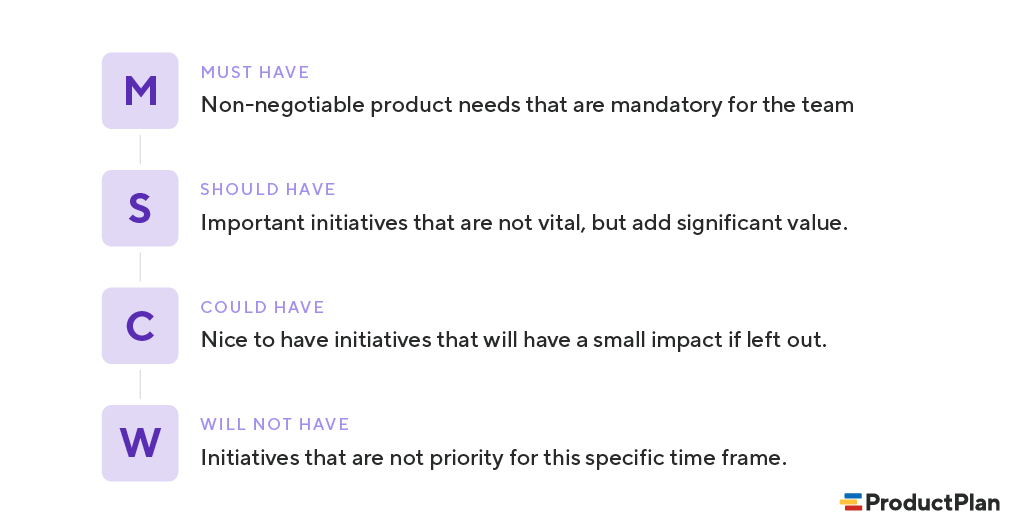
\includegraphics[width=12cm]{figures/MoSCoW-01.png}
\end{figure}
W fazie projektu zostaną wdrożone wszystkie funkcjonalności wymagane, natomiast  
wszelkie pozostałe kategorie zostaną wdrożone w miarę możliwości. Plan 
uwzględnia także cykliczne przeglądy priorytetów aby lepiej dopasować aplikację 
do potrzeb użytkowników i kierunku rozwoju projektu. Zadania rozpisane zostaną 
w metodologii kanban}

\section{\customstylesection{Narzędzia}}
{Podczas projektowania i wdrożenia aplikacji wykorzystane zostaną narzędzia typu
 Open Source oraz komerycjne dostępne nieodpłatnie dla użytkowników 
indywidualnych.}

{Kategoryzacja MoSCoW dla poszczególnych funkcjonalności wykonywana będzie na 
zadaniach zarejstrowanych w tablicy kanban, z wykorzystaniem serwisu Trello 
\cite{Trello}. Model encji w aplikacji zostanie przygotowany w aplikacji StarUML
 \cite{StarUML}. Do stworzenia bazy SQLite \cite{SQLite} posłuży aplikacja 
DB Browser for SQLite \cite{DBBrowser}. Aplikacja Visual Studio Code 
\cite{VSCode} posłuży do pisania kodu w Python \cite{Python} oraz dokumentacji 
w LaTeX \cite{LaTeX}.}

\section{\customstylesection{Techniki}}
{lorem ipsum}

% [REQUIREMENT] 13. Opis głównych klas, metod, obiektów, struktur i algorytmów
% zastosowanych w projekcie (uwzględniając stsosowanie gotowych narzędzi
% obcego autorstwa, w tym open source)
\chapter{\customstylechapter{Opisy metod}}
\section{\customstylesection{Główne klasy projektu}}
{Projekt składa się z warstw bazy danych oraz graficznego interfejsu aplikacji. 
Warstwa bazy przechowuje dane wprowadzone przez użytkownika, na główne klasy 
projektu składają się tabele oraz widoki. Warstwa graficznego interfejsu 
użytkownika odpowiedzialna jest za interakcję z użytkownikiem oraz interakcję
 użytkownika z bazą - prezentację danych przechowywanych w bazie oraz 
wizualizacje danych.}

\section{\customstylesection{Baza danych}}  \label{Baza-danych}

{Podczas tworzenia bazy danych przyjęto kilka podstawowych założeń aby utrzymać 
spójną konwencję nazewniczą pól, tabel i widoków. Dzięki niej interfejs bazy 
jest prostszy a pisanie zapytań bardziej intuicyjne co w ogólnym rozrachunku 
powinno ograniczyć nakład pracy wymagany do wdrożenia dodatkowych funkcji.}

\begin{table}[h]
    \footnotesize
    \begin{tabular}{|p{0.2\linewidth}|p{0.73\linewidth}|}  % | draws verical line
    \hline                  % Draw horizontal line
    % & Defines the breaks in the table 
    \customstyletable{Pole} & \customstyletable{Opis} \\
    \hline
    {ID} & {Identyfikator rekordu}\\
    \hline
    {Comment} & {Komentarz użytkownika}\\
    \hline
    {DateTime} & {Znacznik w standardzie daty międzynarodowej ISO 8601 \cite{ISO 8601}}\\
    \hline
    {Amount} & {Koszt, liczba zmiennoprzecinkowa}\\
    \hline
    {Pole specyficzne} & {Główna informacja, różne nazwy w każdej tabeli (Type,Product)}\\
    \hline
    \end{tabular}
    \caption{Konwencja nazewnicza bazy danych }
\end{table}

\begin{figure}[H]           %requires float package
    \caption{Klasy warstwy bazy danych - tabele}
    \label{fig:Klasy warstwy bazy danych - tabele}
    \centering  
    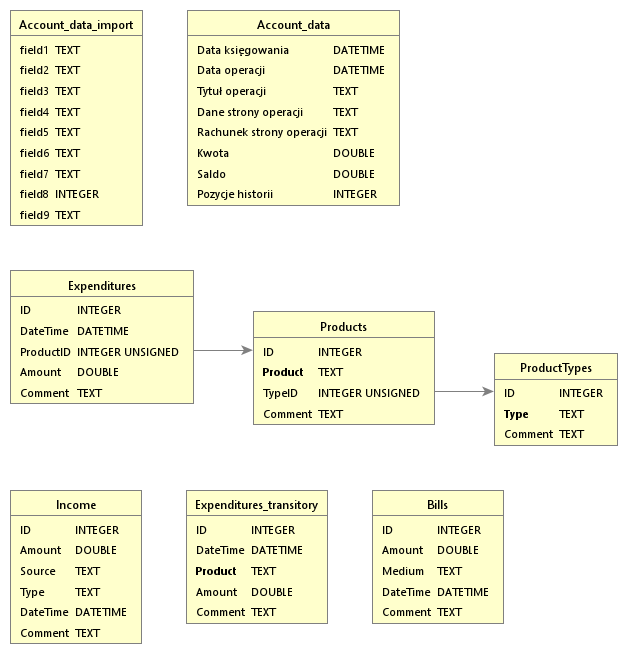
\includegraphics[width=12cm]{figures/Budgeter_Finances-db_Tables.png}
\end{figure}

%-----------------------------TABLES--------------------------------------------
%ADD: Account_data

%[TODO]: Fix - some table span the end of page 
\begin{minipage}{\textwidth}
\begin{lstlisting}[ caption={Tabela ProductTypes},
                    language=SQL,
                    deletekeywords={IDENTITY},
                    deletekeywords={[2]INT},
                    morekeywords={clustered},
                    framesep=8pt,
                    xleftmargin=40pt,
                    framexleftmargin=40pt,
                    frame=tb,
                    framerule=0pt ]
CREATE TABLE [ProductTypes] (
    [ID] 		INTEGER PRIMARY KEY AUTOINCREMENT,
    [Type] 		TEXT 	NOT NULL,
    [Comment] 	TEXT 	DEFAULT NULL
);
\end{lstlisting}
{Tabela ProductTypes zawiera typy produktów zdefiniowane przez użytkownika.}
\end{minipage}

%[TODO] Make function accept 2nd parameter and display caption
%{Tabela ProductTypes zawiera typy produktów zdefiniowane przez użytkownika.}
%\begin{SQLlisting}[{Tabela ProductTypes (v2)}]
%    CREATE TABLE [ProductTypes] (
%        [ID] 		INTEGER PRIMARY KEY AUTOINCREMENT,
%        [Type] 		TEXT 	NOT NULL,
%        [Comment] 	TEXT 	DEFAULT NULL
%    )
%\end{SQLlisting}


\begin{minipage}{\textwidth}
\begin{lstlisting}[ caption={Tabela Products},
    language=SQL,
    deletekeywords={IDENTITY},
    deletekeywords={[2]INT},
    morekeywords={clustered},
    framesep=8pt,
    xleftmargin=40pt,
    framexleftmargin=40pt,
    frame=tb,
    framerule=0pt ]
CREATE TABLE [Products] (
    [ID]        INTEGER PRIMARY KEY AUTOINCREMENT,
    [Product]   TEXT    NOT NULL,
    [TypeID]	INTEGER UNSIGNED, 
    [Comment] 	TEXT    DEFAULT NULL,
FOREIGN KEY([TypeID]) REFERENCES ProductTypes(ID)
);
\end{lstlisting}
{Tabela Products zawiera produkty zdefiniowane przez użytkownika, pole TypeID 
zawiera klucz obcy ID z tabeli ProductTypes.}
\end{minipage}

\begin{minipage}{\textwidth}
\begin{lstlisting}[ caption={Tabela Bills},
    language=SQL,
    deletekeywords={IDENTITY},
    deletekeywords={[2]INT},
    morekeywords={clustered},
    framesep=8pt,
    xleftmargin=40pt,
    framexleftmargin=40pt,
    frame=tb,
    framerule=0pt ]
CREATE TABLE [Bills] (
    [ID]        INTEGER PRIMARY KEY AUTOINCREMENT,
    [Amount]    DOUBLE,
    [Medium]    TEXT,
    [DateTime]  DATETIME,
    [Comment]   TEXT DEFAULT NULL
);
\end{lstlisting}
{Tabela Bills zawiera wydatki stałe wprowadzone przez użytkownika.}
\end{minipage}

\begin{minipage}{\textwidth}
\begin{lstlisting}[ caption={Tabela Income},
    language=SQL,
    deletekeywords={IDENTITY},
    deletekeywords={[2]INT},
    morekeywords={clustered},
    framesep=8pt,
    xleftmargin=40pt,
    framexleftmargin=40pt,
    frame=tb,
    framerule=0pt ]
CREATE TABLE [Income] (
	[ID] 		INTEGER PRIMARY KEY AUTOINCREMENT,
	[Amount]	DOUBLE,
	[Source]	TEXT,
	[Type]		TEXT,
	[DateTime]	DATETIME,
	[Comment]	TEXT DEFAULT NULL
);
\end{lstlisting}
{Tabela Income zawiera wpływy wprowadzone przez użytkownika.}
\end{minipage}

\begin{minipage}{\textwidth}
\begin{lstlisting}[ caption={Tabela Expenditures},
    language=SQL,
    deletekeywords={IDENTITY},
    deletekeywords={[2]INT},
    morekeywords={clustered},
    framesep=8pt,
    xleftmargin=40pt,
    framexleftmargin=40pt,
    frame=tb,
    framerule=0pt ]
CREATE TABLE [Expenditures] (
	[ID]	INTEGER,
	[DateTime]	DATETIME,
	[ProductID]	INTEGER UNSIGNED,
	[Amount]	DOUBLE,
	[Comment]	TEXT DEFAULT NULL,
	PRIMARY KEY([ID] AUTOINCREMENT),
	FOREIGN KEY([ProductID]) REFERENCES [Products]([ID])
);
\end{lstlisting}
{Tabela Expenditures zawiera wydatki wprowadzone przez użytkownika.}
\end{minipage}

\begin{minipage}{\textwidth}
\begin{lstlisting}[ caption={Tabela Expenditures\_transitory},
    language=SQL,
    deletekeywords={IDENTITY},
    deletekeywords={[2]INT},
    morekeywords={clustered},
    framesep=8pt,
    xleftmargin=40pt,
    framexleftmargin=40pt,
    frame=tb,
    framerule=0pt ]
CREATE TABLE [Expenditures_transitory] (
	[ID]	INTEGER,
	[DateTime]	DATETIME,
	[ProductID]	INTEGER UNSIGNED,
	[Amount]	DOUBLE,
	[Comment]	TEXT DEFAULT NULL,
	PRIMARY KEY([ID] AUTOINCREMENT),
	FOREIGN KEY([ProductID]) REFERENCES [Products]([ID])
);
\end{lstlisting}
{Tabela Expenditures\_transitory tymczasowo przechowuje wydatki wprowadzone przez
 użytkownika. Dane któe które się w niej znajdują są sprawdzane pod względem 
 poprawności, po czym poprawne dane są przenoszone do tabeli Expenditures i 
 usuwane z Expenditures\_transitory. Na dłużej pozostają w niej tylko dane które 
 użytkownik musi poprawić.}
\end{minipage}


%------------------------------VIEWS--------------------------------------------
%[TODO]: Add Ledger_comparison, MonthlyCharge

\begin{minipage}{\textwidth}
\begin{lstlisting}[ caption={Widok Expenditures\_Enriched},
    language=SQL,
    deletekeywords={IDENTITY},
    deletekeywords={[2]INT},
    morekeywords={clustered},
    framesep=8pt,
    xleftmargin=40pt,
    framexleftmargin=40pt,
    frame=tb,
    framerule=0pt ]
CREATE VIEW [Expenditures_Enriched] AS
SELECT  [EXP].[ID]          as ID,
        [EXP].[DateTime]    as DateTime,
        [EXP].[Amount]      as Amount,
        [PRD].[Product]     as Product,
        [PTY].[Type]        as Type,
        [EXP].[Comment]     as Comment
FROM  [Expenditures]            [EXP]
LEFT JOIN [Products]            [PRD]	
    ON [EXP].[ProductID]=[PRD].[ID]
LEFT JOIN [ProductTypes]        [PTY]
    ON [PRD].[TypeID]=[PTY].[ID]
ORDER BY DateTime;
\end{lstlisting}
{Widok Expenditures\_Enriched prezentuje użytkownikowi czytelne dane z tabeli 
Expenditures wzbogacone o zdefiniowane produkty z tabeli Products i typy z 
tabeli ProductTypes.}
\end{minipage}

\begin{minipage}{\textwidth}
\begin{lstlisting}[ caption={Widok ProductTypeSummary},
    language=SQL,
    deletekeywords={IDENTITY},
    deletekeywords={[2]INT},
    morekeywords={clustered},
    framesep=8pt,
    xleftmargin=40pt,
    framexleftmargin=40pt,
    frame=tb,
    framerule=0pt ]
CREATE VIEW [ProductTypeSummary] AS
SELECT 
	*
	,(CASE WHEN ([Bought Times]>(
                SELECT 
                    AVG([Bought Times]) AS [Average] 
                FROM (SELECT
                    [Type]
                    ,Round(SUM([Amount]), 2)AS [Amount]
                    ,COUNT([DateTime])  AS [Bought Times]
                    ,MAX(DateTime)      AS [LastBought]
                    ,MIN(DateTime)  AS [FirstBought]
                    FROM [Expenditures_Enriched]
                    GROUP BY [Type]
                    ORDER BY [Bought Times] DESC)))
	then 'Common' else 'Uncommon' end) as [Common]
FROM (SELECT
        [Type]
        ,Round(SUM([Amount]), 2) AS [Amount]
        ,COUNT([DateTime])       AS [Bought Times]
        ,MAX(DateTime)           AS [LastBought]
        ,MIN(DateTime)           AS [FirstBought]
    FROM [Expenditures_Enriched]
    GROUP BY [Type]
    ORDER BY [Bought Times] DESC);
\end{lstlisting}
{Widok ProductTypeSummary podsumowujący dla użytkownika dane o typach produktów.}
\end{minipage}

\begin{minipage}{\textwidth}
    \begin{lstlisting}[ caption={Widok ProductSummary},
        language=SQL,
        deletekeywords={IDENTITY},
        deletekeywords={[2]INT},
        morekeywords={clustered},
        framesep=8pt,
        xleftmargin=40pt,
        framexleftmargin=40pt,
        frame=tb,
        framerule=0pt ]
CREATE VIEW [ProductSummary] AS
SELECT
    *
    ,(CASE WHEN ([Bought Times]>(
        SELECT AVG([Bought Times]) AS [Average] 
        FROM (SELECT
                [Product]
                ,Round(SUM([Amount]), 2) AS [Amount]
                ,COUNT([DateTime])       AS [Bought Times]
                ,MAX(DateTime)           AS [LastBought]
                ,MIN(DateTime)           AS [FirstBought]
                FROM [Expenditures_Enriched]
                GROUP BY [Product]
                ORDER BY [Bought Times] DESC)))
	then 'Common' else 'Uncommon' end) as [Common]
FROM (SELECT
        [Product]
        ,Round(SUM([Amount]), 2)AS [Amount]
        ,COUNT([DateTime])      AS [Bought Times]
        ,MAX(DateTime)          AS [LastBought]
        ,MIN(DateTime)          AS [FirstBought]
     FROM [Expenditures_Enriched]
     GROUP BY [Product]
     ORDER BY [Bought Times] DESC);
\end{lstlisting}
{Widok ProductSummary podsumowujący dla użytkownika statystyki produktów.}
\end{minipage}


\begin{minipage}{\textwidth}
\begin{lstlisting}[ caption={Widok MonthlyExpenditures},
    language=SQL,
    deletekeywords={IDENTITY},
    deletekeywords={[2]INT},
    morekeywords={clustered},
    framesep=8pt,
    xleftmargin=40pt,
    framexleftmargin=40pt,
    frame=tb,
    framerule=0pt ]
CREATE VIEW [MonthlyExpenditures] AS
SELECT 
    SUBSTR([DateTime], 1, 7)    as [Month]
    ,SUM([Amount])              as [Amount]
FROM [Expenditures_Enriched]
GROUP BY [Month]
ORDER BY [Month];
\end{lstlisting}
{Widok MonthlyExpenditures podsumowujący dla użytkownika dane o miesięcznych 
wydatkach.}
\end{minipage}

\begin{minipage}{\textwidth}
\begin{lstlisting}[ caption={Widok MonthlyBills},
    language=SQL,
    deletekeywords={IDENTITY},
    deletekeywords={[2]INT},
    morekeywords={clustered},
    framesep=8pt,
    xleftmargin=40pt,
    framexleftmargin=40pt,
    frame=tb,
    framerule=0pt ]
CREATE VIEW [MonthlyBills] AS
SELECT 
    SUBSTR([DateTime], 1, 7)    as [Month]
    ,SUM([Amount])              as [Amount]
FROM [Bills]
GROUP BY [Month]
ORDER BY [Month];
\end{lstlisting}
{Widok MonthlyBills podsumowujący dla użytkownika dane o rachunkach bieżących 
w rozrachunku miesięcznym zawartych w tabeli Bills.}
\end{minipage}

\begin{minipage}{\textwidth}
\begin{lstlisting}[ caption={Widok MonthlyIncome},
    language=SQL,
    deletekeywords={IDENTITY},
    deletekeywords={[2]INT},
    morekeywords={clustered},
    framesep=8pt,
    xleftmargin=40pt,
    framexleftmargin=40pt,
    frame=tb,
    framerule=0pt ]
CREATE VIEW [MonthlyIncome] AS
SELECT
	SUBSTR([DateTime], 1, 7)				as Month
	,SUM([Amount])							as Amount
FROM 	[Income]
GROUP BY [Month]
ORDER BY [Month];
\end{lstlisting}
{Widok MonthlyIncome podsumowujący dla użytkownika dane o przychodach w ujęciu 
miesięcznym.}
\end{minipage}

\begin{minipage}{\textwidth}
\begin{lstlisting}[ caption={Widok MonthlyBilance},
    language=SQL,
    deletekeywords={IDENTITY},
    deletekeywords={[2]INT},
    morekeywords={clustered},
    framesep=8pt,
    xleftmargin=40pt,
    framexleftmargin=40pt,
    frame=tb,
    framerule=0pt ]
CREATE VIEW [MonthlyBilance] AS 
SELECT 
    Strftime('%Y-%m', [DateTime])   as [Month],
    Strftime('%Y',    [DateTime])   as [Year],
    ROUND(SUM([Amount]), 2)         as [Income]
    --Previous_month_income - (bills + expenditures)
FROM (SELECT 
        DATE(Strftime('%Y-%m-01', [DateTime]),[-1 month]) as [DateTime],
        [Amount]  
      FROM [Income]
      UNION SELECT
                [DateTime], 
                -([Amount]) 
            FROM [Expenditures_Enriched]
      UNION SELECT
                [DateTime],
                -([Amount])
            FROM [Bills])
 GROUP BY [Month]
 ORDER BY [Month] DESC;
\end{lstlisting}
{Widok MonthlyBilance podsumowujący dla użytkownika bilans miesięczny wydatków i
 wpływów w formie pojedynczej liczby.}
\end{minipage}

\begin{minipage}{\textwidth}
\begin{lstlisting}[ caption={Widok Monthly\_common\_products},
    language=SQL,
    deletekeywords={IDENTITY},
    deletekeywords={[2]INT},
    morekeywords={clustered},
    framesep=8pt,
    xleftmargin=40pt,
    framexleftmargin=40pt,
    frame=tb,
    framerule=0pt ]
CREATE VIEW [Monthly_common_products] AS
SELECT * 
FROM (
    SELECT  Strftime('%Y-%m', [DateTime])   AS [Month],
            [Product],
            COUNT([Product])                AS [Items], 
            SUM([Amount])                   AS [Sum]
    FROM [Expenditures_Enriched]
    GROUP BY [Product], [Month]
    ORDER BY [Month] DESC, [Sum] DESC
) WHERE [Items]>=4;
\end{lstlisting}
{Widok Monthly\_common\_products podsumowujący dla użytkownika dane o najczęściej 
kupowanych produktach danego miesiąca. Uwzględnia wyłącznie produkty które 
zakupiono 4 razy - liczba ta została wybrana arbitralnie metodą kolejnych 
przybliżeń aby otrzymać zadowalający wynik.}
\end{minipage}

\begin{minipage}{\textwidth}
\begin{lstlisting}[ caption={Widok Monthly\_Expenditures\_by\_Type},
    language=SQL,
    deletekeywords={IDENTITY},
    deletekeywords={[2]INT},
    morekeywords={clustered},
    framesep=8pt,
    xleftmargin=40pt,
    framexleftmargin=40pt,
    frame=tb,
    framerule=0pt ]
CREATE VIEW [Monthly_Expenditures_by_Type] AS 
SELECT	Strftime('%Y-%m', [DateTime]) as [Month],
        Strftime('%Y',    [DateTime]) as [Year],
        ROUND(SUM([Amount]), 2)       as [Sum],
        [Type]
FROM (SELECT 
        [DateTime], 
        [Type], 
        [Amount] 
      FROM [Expenditures_Enriched])
GROUP BY [Type], [Month]
ORDER BY [Month] DESC, [Sum] DESC;
\end{lstlisting}
{Widok Monthly\_Expenditures\_by\_Type podsumowujący dla użytkownika dane o 
typach produktów w ujęciu miesięcznym.}
\end{minipage}

\begin{minipage}{\textwidth}
\begin{lstlisting}[ caption={Widok Temp\_check},
    language=SQL,
    deletekeywords={IDENTITY},
    deletekeywords={[2]INT},
    morekeywords={clustered},
    framesep=8pt,
    xleftmargin=40pt,
    framexleftmargin=40pt,
    frame=tb,
    framerule=0pt ]
CREATE VIEW [Temp_check] 
    (Temp_ID, Temp_Product, Product_ID)
AS
SELECT *
FROM (SELECT 
        Expenditures_transitory.ID      as [Temp_ID],
        Expenditures_transitory.Product as [Temp_Product],
        Products.ID                     as [Product_ID]
      FROM [Expenditures_transitory]
      LEFT OUTER JOIN [Products]
      ON [Expenditures_transitory].[Product]==[Products].[Product]
)
WHERE [Product_ID] IS NULL;
\end{lstlisting}
{Widok Temp\_check służy użytkownikowi do weryfikacji poprawności wprowadzonych 
danych.}
\end{minipage}

\begin{minipage}{\textwidth}
\begin{lstlisting}[ caption={Widok Products\_to\_fix},
    language=SQL,
    deletekeywords={IDENTITY},
    deletekeywords={[2]INT},
    morekeywords={clustered},
    framesep=8pt,
    xleftmargin=40pt,
    framexleftmargin=40pt,
    frame=tb,
    framerule=0pt ]
CREATE VIEW [Products_to_fix] AS
SELECT *
FROM [Expenditures_Enriched]
WHERE [Product] IN (NULL,
                    'UNKNOWN')
    OR [Comment] LIKE '%[TODO]%';
\end{lstlisting}
{Widok Products\_to\_fix zawiera dane wprowadzone przez użytkownika któe 
zostały zaakceptowane jednak wymagają poprawy. Rozpoznawane są po specjalnych
 wartościach w polu PRODUCT lub oznaczeniu [TODO] w komentarzu.}
\end{minipage}

%------------------------- Application layer ----------------------------------- 

\section{\customstylesection{Graficzny interfejs użytkownika}} \label{GUI}

\begin{figure}[H]           %requires float package
    \caption{Wizualizacja danych wersja 2}
    \label{fig:Wizualizacja danych wersja 2}
    \centering  
    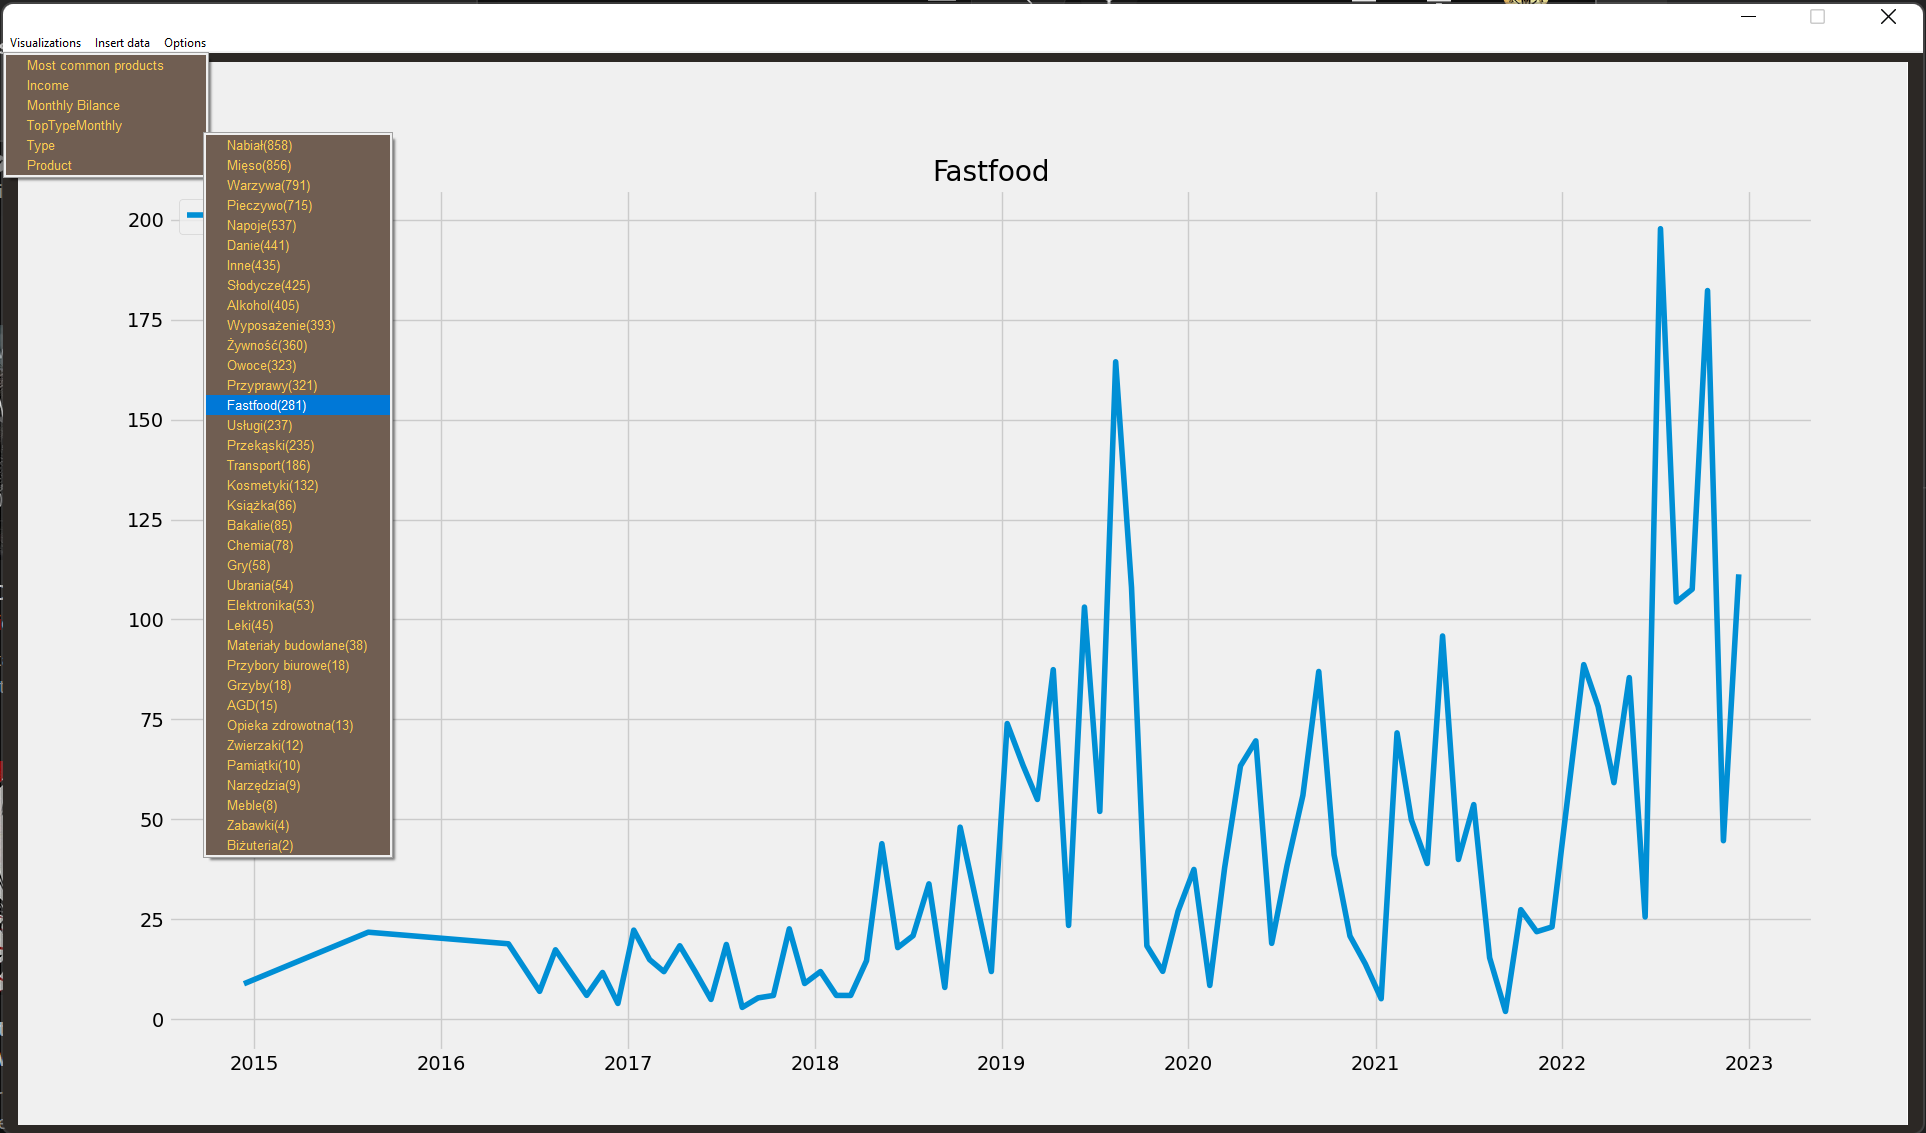
\includegraphics[width=12cm]{figures/Interface_v0.2.png}
\end{figure}
\section{\customstylesection{Metody projektu}}
{lorem ipsum}

\section{\customstylesection{Obiekty projektu}}
{lorem ipsum}

\section{\customstylesection{Struktury projektu}}
{lorem ipsum}

\section{\customstylesection{Algorytmy projektu}}
{lorem ipsum}

% [REQUIREMENT] 22. Bibliografia - wykaz wszystkich źródeł
\begin{thebibliography} {books}
\bibitem{wiki_ekonomia} Wikipedia, Nauki Ekonomiczne \raggedright\url{
    https://pl.wikipedia.org/wiki/Nauki_ekonomiczne}
\bibitem{gus_sytuacja_budzetowa} Główny Urząd Statystyczny \raggedright\url{
    https://stat.gov.pl/obszary-tematyczne/warunki-zycia/dochody-wydatki-i-warunki-zycia-ludnosci/sytuacja-gospodarstw-domowych-w-2021-r-w-swietle-badania-budzetow-gospodarstw-domowych,3,21.html}
\bibitem{o24_budzetowanie} Opcje24, Budzetowanie \raggedright\url{
    https://www.opcje24h.pl/budzetowanie-przewodnik-planowanie-budzetu/}
\bibitem{MOSCOW} Product Plan, MOSCOW Prioritetization \raggedright\url{
    https://www.productplan.com/glossary/moscow-prioritization/}
\bibitem{MVP} Wikipedia, Minimal Viable Product \raggedright\url{
    https://en.wikipedia.org/wiki/Minimum_viable_product}
\bibitem{ISO 8601} NASA.gov, A summary of the international standard date and time notation \raggedright\url{
    https://fits.gsfc.nasa.gov/iso-time.html}
\bibitem{CSV} Y. Shafranovich, SolidMatrix Technologies, Inc., Common Format and MIME Type for Comma-Separated Values (CSV) Files \raggedright\url{
    https://www.rfc-editor.org/rfc/rfc4180}
\bibitem{SQLite} sqlite.org, SQLite \raggedright\url{
    https://www.sqlite.org/index.html}
\bibitem{Python} python.org, Python \raggedright\url{
    https://www.python.org/}
\bibitem{PySimpleGUI} pysimplegui.org, PySimpleGUI Python GUIs for Humans \raggedright\url{
    https://www.pysimplegui.org/en/latest/}
\bibitem{JSON} json.org, Introducing JSON \raggedright\url{
    https://www.json.org/json-en.html}
\bibitem{Python_read-file} pythonspot.com, Python tutorials, How to Read a File in Python \raggedright\url{
    https://pythonspot.com/read-file/}
\bibitem{Trello} Atlassian, Trello.com \raggedright\url{
    https://trello.com/}
\bibitem{StarUML} MKLabs Co.,Ltd, StarUML \raggedright\url{
    https://staruml.io/}
\bibitem{LaTeX} The LaTeX Project \raggedright\url{
    https://www.latex-project.org/}
\bibitem{VSCode} Microsoft, Visual Studio Code \raggedright\url{
    https://code.visualstudio.com/}   
\bibitem{DBBrowser} Public domain, DB Browser for SQLite \raggedright\url{
    https://sqlitebrowser.org/}   
\end{thebibliography}

% [REQUIREMENT] 21. Spisy ilustracji (spis obiektów graficznych, diagramów, tabel...)
\listoffigures
\listoftables
\lstlistoflistings

\end{document}


% ------------------------------ Docummentation -------------------------------

% ------ Project deadline 2023-01-29 ------------------------------------------
% ------ Part 1: Due 2022-10-21 

% ------ Part 2: Due 2022-11-18 
% [REQUIREMENT] 15. Przebieg uruchamiania projektu (być może na różnych 
% platformach, konfiguracjach...)
% [REQUIREMENT] 16. Przebieg testowania projektu (rodzaje i metody przeprowadzonych
% testów)
% [REQUIREMENT] 17. Wnioski z przebiegu testowania (wykryte defekty, wrażliwość
% na specyficzne dane, błędy ukryte i niewidoczne dla użytkownika, sytuacje
% niejednoznaczne itp.)
% [REQUIREMENT] 18. Konserwacja systemu
% [REQUIREMENT] 19. Podsumowanie i alternatywne sposoby stworzenia projektu
% (po zdobytym doświadczeniu, przy dostępie do innych narzędzi, przy innej wizji...)
% [REQUIREMENT] 20. Dokumentacja dla użytkownika (Podręczni kużytkownika)
% [REQUIREMENT] 20.1. Przeznaczenie i główne możliwości systemu
% [REQUIREMENT] 20.2. Podstawowe wymagania
% [REQUIREMENT] 20.3. Opis instalacji/uruchamiania
% [REQUIREMENT] 20.4. Kompletny opis działających funkcji (menu, opis interface...),
% formatów danych, obsługi błędów użytkowania, zakresów danych 
% [REQUIREMENT] 20.5. Podręcznik administratora/użytkownika systemu/gościa
% [REQUIREMENT] 20.6. Spostrzeżenia i zalecenia do użytkowania projektu
% [REQUIREMENT] 20.7. Wykryte błędy w działaniu


% DONE
% [REQUIREMENT] 1. Strona tytułowa
% [REQUIREMENT] 2. Spis treści
% [REQUIREMENT] 3. Wprowadzenie do tematyki projektu
% [REQUIREMENT] 4. Zamierzony cel projektu
% [REQUIREMENT] 5. Wstępne założenia i uwarunkowania, w których 
% projekt będzie powstawał  -----------------------
% [REQUIREMENT] 6. Założone ograniczenia (ramy czasowe, umiejętności) 
% i możliwość ewaluacji projektu
% [REQUIREMENT] 7. Chronologiczny plan pracy (ujecie przyjetego modelu 
% projektowania i faz projektowania)
% [REQUIREMENT] 8. POWYŻSZĄ CZĘŚĆ DOKUMENTACJI ODDAJEMY PRZED REALIZACJĄ PROJEKTU
% [REQUIREMENT] 9. Wymagania funkcjonalne (szczegółowey wykaz wszystkich funkcji 
% oprogramowania) jakie funkcjonalności oprogramowania chcemy dostarczyć, można 
% nie zdążyć z dostarczeniem części, lub dopisać dodatkowe dodane w trakcie
% [REQUIREMENT] 10. Wymagania niefunkcjonalne
% [REQUIREMENT] 10.1. Sprzętowe (w różnych wariantach, w tym dostęp do 
% koniecznych lub alternatywnych nośników danych i peryferiów)
% [REQUIREMENT] 10.2. Systemowe (systemy operacyjne, zainstalowane środowiska, 
% platformy, pakiety, biblioteki, sterowniki)
% [REQUIREMENT] 10.3. Organizacyjne (np. organizacja pracy z systemem, warunki 
% poprawnej pracy przy większej liczbie użytkownikó, stanowisk, obciążeniu sieci,
% konieczność zapewnienia realnego czasu dostępu itd.itp.)
% [REQUIREMENT] 11. Wymagania dotyczące danych (wykaz tabel, relacji, 
% typy i rozmiary pól z uzasadnieniem, inne rodzaje danych w tym logi, hasła)
% [REQUIREMENT] 12. Metody pracy, narzędzia i techniki
% [REQUIREMENT] 13. Opis głównych klas, metod, obiektów, struktur i algorytmów
% zastosowanych w projekcie (uwzględniając stsosowanie gotowych narzędzi
% obcego autorstwa, w tym open source)
% [REQUIREMENT] 14. POWYŻSZĄ CZĘŚĆ DOKUMENTACJI ODDAJEMY W TRAKCIE TWORZENIA
% [REQUIREMENT] 23. Przypisy dolne, stopki (nr stron), nagłówki...
% [REQUIREMENT] 22. Bibliografia - wykaz wszystkich źródeł
% [REQUIREMENT] 21. Spisy ilustracji (spis obiektów graficznych, diagramów, tabel...)

% --------------------------------- Purgatory ----------------------------------
% Orphaned snippets of texts placed here untill you decide what to do with them
% -----
% domowym i udostępnienie podstawowych informacji finansowych Niestety jedak 
% zakres wiedzy w zakresie finansów którą posiada przeciętny obywatel jest dość 
% niski, w połączeniu z obecnie panującą trudną sytuacją gospodarczą w wielu 
% miejscach na świecie część ludzi nie radzi sobie z dopinaniem budżetu 
% domowego. Jest to jednak dziedzina dość skomplikowana, a tym samym trudna dla 
% przeciętnego obywatela.